\chapter{Introdución}
\label{chap:introducion}

Este proxecto céntrase no desenvolvemento de \textbf{SintromApp}, unha aplicación móbil destinada a mellorar o seguimento do tratamento anticoagulante, ofrecendo unha alternativa dixital aos métodos físicos tradicionais.

\section{Contexto}

En España, preto de 800.000 persoas reciben tratamento con anticoagulantes. Concretamente, en Galicia estímase que uns 50.000  \cite{PacientesAnticoaguladosAnis} pacientes están baixo este tipo de medicación. Pese a importancia vital deste tratamento, a súa xestión diaria é moi arcaica. O paciente ten que depender \textbf{exclusivamente} dun informe en papel onde se detallan as doses diarias (Figura \ref{fig:follasintrom}).

Este formato físico é \textbf{moi fráxil}, xa que o papel pode perderse ou estragarse, o que deixa ao paciente sen o medio imprescindible para poder realizar correctamente as tomas pautadas, provocando que teña que desprazarse ao centro de saúde. Ademais, a xestión manual do tratamento pode aumentar o risco de esquecementos nas tomas.

Aínda que o informe do tratamento tamén se atopa en formato dixital a través da plataforma eSaude, o acceso a esta pode resultar bastante complexo para algúns pacientes, especialmente no caso das persoas maiores, xa que \textbf{ é imprescindible  dispoñer dun certificado dixital, chave365 ou DNI electrónico.}

Unha das principais complexidades deste tratamento é que a dose non é fixa. Como se pode observar no informe da Figura \ref{fig:follasintrom}, a pauta vai variando dependendo do día da semana, o que obriga ao paciente a realizar un esforzo para asegurarse que a dose que vai a tomar é a correcta e se corresponde co día concreto. 

Un fallo na dosificación pode ter consecuencias moi negativas na saúde do paciente. O Sintrom é un fármaco cunha marxe terapéutica moi estreita, o que implica que un pequeno cambio na dose pode provocar hemorraxias graves ou trombos. Un erro de interpretación da táboa de doses (como por exemplo tomar a dose doutro día en lugar da do día que toca), ou o esquecemento da toma, poden poñer en risco a saúde do paciente. 

Outro inconveniente do formato físico é a dificultade para consultar a evolución do tratamento ao longo do tempo. O paciente adoita tirar os informes vellos, perdendo a información de como evoluciona o \gls{inr} ou as súas doses nos últimos meses. A dixitalización permite manter un histórico que facilita ao paciente unha perspectiva para ver os seus avances.

Ademais, o seguimento manual carece de mecanismos de notificación ou confirmación das tomas, o que limita a capacidade de supervisión por parte dos coidadores. Isto xera incerteza e preocupación, xa que non poden saber se o paciente tomou a dose sen falar directamente con el, quen á súa vez pode non lebrar se a tomou ou non. Como consecuencia, aumenta o risco de non actuar a tempo ante un esquecemento.

\begin{figure}[h!]
\centering
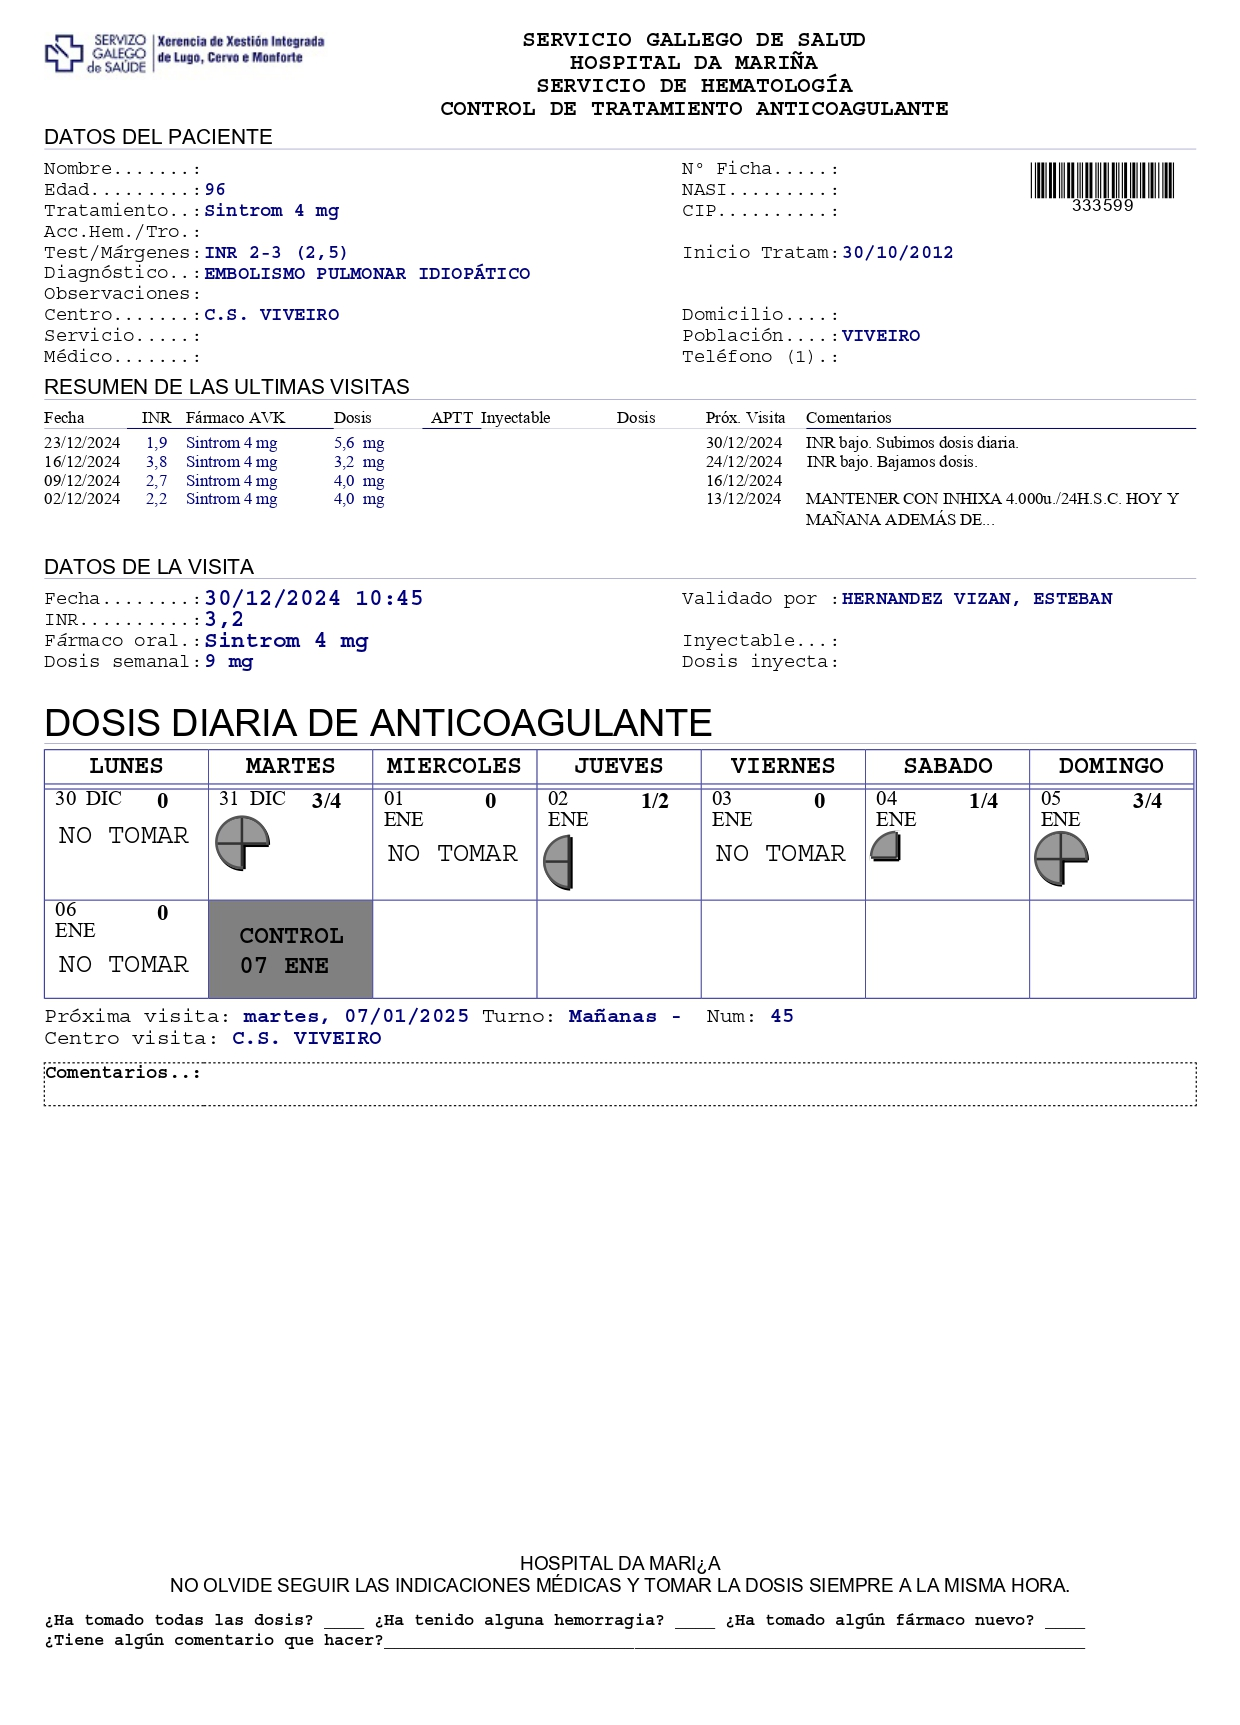
\includegraphics[width=0.7\textwidth]{imaxes/Introducion/IMAXE_SINTROM.jpg}
\caption{Exemplo de folla de tratamento}
\label{fig:follasintrom}
\end{figure}

\section{Motivación}

Este proxecto nace coa premisa de achegar seguridade ao tratamento e maior tranquilidade tanto aos pacientes como aos seus familiares e coidadores. Como se expuxo na sección anterior, no sistema actual, moitos pacientes viven coa constante preocupación de perder ou estragar a folla de tratamento. Ademais deben interpretar a pauta diaria a partir dunha táboa que pode resultar complexa e difícil de ler debido ao reducido tamaño de letra. Ao mesmo tempo, o proxecto busca aliviar os familiares ou coidadores, que adoitan vivir coa incerteza de non saber se a toma foi realizada correctamente.

A motivación principal deste proxecto é aproveitar as posibilidades que nos ofrecen os dispositivos móbiles para simplificar e reducir estes riscos ao mínimo. Para iso, proponse unha ferramenta \textbf{sinxela e intuitiva}, accesible para calquera persoa usuaria. A aplicación pretende dixitalizar a información do tratamento a partir dunha simple fotografía da folla de prescrición, permitindo extraer automaticamente toda a información necesaria e xerar recordatorios diarios para o paciente.

Ademais, incorpórase un sistema de confirmación das tomas. O paciente pode marcar na aplicación cando realiza a toma da dose que lle corresponde e, no caso de que esta non sexa rexistrada nun intervalo de tempo, o sistema envía unha notificación a un familiar ou coidador para que poida comprobar a situación e actuar no caso de que sexa necesario.

Deste modo, a aplicación busca transformar un proceso actualmente manual e dependente do papel nun sistema dixital e accesible que mellore a seguridade do paciente e facilite o seguimento do tratamento anticoagulante no día a día.

\section{Obxectivos}

O obxectivo principal deste proxecto é desenvolver unha aplicación móbil multiplataforma que facilite a xestión diaria do tratamento con Sintrom. Para logralo, establécense os seguintes obxectivos:
\begin{itemize}
    \item\textbf{ Eliminar a dependencia do papel:} Ao dixitalizar o informe, a información estará sempre dispoñible no móbil, evitando desprazamentos ao centro médico no caso de perda ou estragamento do documento orixinal.
    \item \textbf{Automatizar a entrada de datos mediante técnicas de procesado de imaxe:} Substituír a carga manual de información por un sistema que lea a imaxe da folla médica, reducindo os posibles erros ao copiar as doses.
    \item \textbf{Mellorar a seguridade nas tomas:} Reducir o risco de esquecementos mediante recordatorios programados e un sistema de avisos automáticos aos coidadores.
    \item \textbf{Facilitar o control a pacientes e coidadores: } Proporcionar un seguimento detallado das tomas e ofrecer un rexistro visual e sinxelo sobre a evolución histórica dos valores de \gls{inr} e da dose.
    \item \textbf{Garantir a privacidade dos datos:} Protexer a información médica evitando a súa persistencia nos servidores da aplicación, almacenando de forma segura os datos sensibles no dispositivo e cifrando a nivel de aplicación as mensaxes intercambiadas entre os dispositivos vinculados.
\end{itemize}

\section{Estudo de mercado}
Para avaliar a viabilidade deste proxecto, realizouse unha análise das solucións dispoñibles actualmente para o seguimento do tratamento de anticoagulante oral. A análise realizada mostra que o mercado se divide en dúas grandes categorías, aplicacións xenéricas de medicación e aplicacións específicas para Simtrom.


\subsection{Aplicacións xenéricas}
\label{subsec:aplicacións_xenericas}
Nesta categoría inclúense ferramentas que permiten a xestión xeral da medicación, permitindo crear recordatorios e rexistrar diferentes fármacos. 

Algunhas das app máis populares desta categoría son, por exemplo, \textit{Medisafe} \cite{AppMedisafe} ou \textit{MyTherapy} \cite{AppMyTherapy}. As capturas de ambas aplicacións recóllense no Apéndice~\ref{app:capturas-estudo-mercado}. Malia ser aplicacións bastante completas para o control de medicación xeral, non están adaptadas ás características específicas do tratamento anticoagulante. Algunhas das principais limitacións atopadas nestas solucións son:
\begin{itemize}
    \item \textbf{Xestión de pautas variables:} Estas aplicacións están deseñadas só para tratamentos recorrentes ou con doses fixas (ex. unha pastilla cada 8 horas, media pastilla cada 3 horas, unha pastilla diaria...). Se quixésemos empregar este tipo de apps para levar o control do tratamento de Sintrom teríamos que configurar, por exemplo, para unha folla cunha pauta de 7 días cunha dose cambiante diariamente, sete alarmas distintas con doses diferentes, o que induce ao erro.
    \item \textbf{Carga manual de datos:}  O usuario debe escribir cada medicamento e dose. Para unha persoa de avanzada idade isto resulta complexo e pode inducir a erros, creando unha gran barreira de uso da app.
\end{itemize}

\subsection{Aplicacións especializadas}
Existen algunhas solucións deseñadas especificamente para este tratamento como por exemplo:
\begin{itemize}
    \item \textbf{AnticoagulApp} \cite{AppAnticoagulApp}: Esta é unha aplicación lanzada pola \textit{Sociedade Española de Cardioloxía} que permite rexistrar o \gls{inr}, as doses e ofrece consellos de saúde. Se ben mellora as alternativas xenéricas ao adaptarse ás doses variables, mantén a barreira principal, xa que require que o usuario rexistre as doses manualmente. Non ten capacidade de interpretar documentos físicos, obrigando ao paciente a ler e transcribir a folla do médico. A súa interface pode consultarse na Figura~\ref{fig:AppAnticoagulApp} do Apéndice~\ref{app:capturas-estudo-mercado}. \footnote{Durante o período de redacción da memoria deste traballo esta aplicación non está dispoñible xa que se atopa en proceso de actualizacións.}
    \item \textbf{INR Diary} \cite{AppINRDiary}:  Aínda que permite un rexistro detallado do \gls{inr} e das doses tomadas, a entrada de datos segue a ser completamente manual. Ademais esta aplicación é de pago, o que supón unha barreira económica engadida que limita a súa accesibilidade para gran parte dos pacientes.  A súa interface móstrase na Figura~\ref{fig:AppINRDiary} do Apéndice~\ref{app:capturas-estudo-mercado}.
\end{itemize}

\FloatBarrier

\begin{table}[hp!]
  \centering
  \caption{Comparativa de funcionalidades das aplicacións existentes e da nosa solución}
  \rowcolors{2}{white}{udcgray!25}
  \resizebox{\textwidth}{!}{
  \begin{tabular}{c|c|c|c|c}
  \rowcolor{udcpink!25}
  \textbf{Funcionalidade} & \textbf{App Xenérica} & \textbf{AnticoagulApp} & \textbf{INR Diary} & \textbf{SintromApp} \\\hline
  \textit{Recordatorios Sonoros} & Si & Si & Si & Si \\
  \textit{Histórico INR} & Non & Si & Si & Si \\
  \textit{Entrada por técnicas de procesado de imaxe} & Non & Non & Non & Si \\
  \textit{Aviso a coidadores} & Algunhas & Non & Non & Si \\
  \textit{Dose diaria variable} & Manual & Manual & Manual & Automática \\
  \end{tabular}
  }
  \label{tab:comparativa}
\end{table}


Como se pode observar na Táboa \ref{tab:comparativa}, as solucións existentes presentan limitacións importantes no contexto específico do tratamento con Sintrom. Ningunha das aplicacións analizadas permite extraer automaticamente a información a partir dunha folla de prescrición médica, delegando a responsabilidade da carga de datos no paciente.

Para dar resposta a estas limitacións, a nosa proposta introduce unha solución centrada na automatización e na adaptación ás necesidades reais dos pacientes anticoagulados. Concretamente, a ferramenta \textbf{desmarcarase} das alternativas actuais baseándose nos seguintes piares:

\begin{itemize}
    \item \textbf{Automatización mediante procesado de imaxe:} A aplicación \textbf{é capaz} de ler e interpretar a folla do SERGAS mediante a cámara do dispositivo, eliminando por completo a necesidade de que o paciente teña que teclear as súas doses.
    \item \textbf{Adaptación nativa a pautas variables:} A lóxica do sistema \textbf{está deseñada} especificamente para o Sintrom, xestionando de forma autónoma as doses cambiantes de cada día sen requirir múltiples configuracións manuais.
    \item \textbf{Rede de seguridade familiar:} \textbf{Intégrase} un sistema de notificacións que avisará automaticamente aos coidadores ou familiares en caso de que o paciente se esqueza da súa toma diaria.
    \item \textbf{Foco na fenda dixital:} Para romper as barreiras de adopción tecnolóxica, a interface \textbf{conta} cun ``modo sinxelo'' pensado especificamente para persoas de avanzada idade.
\end{itemize}

Con este conxunto de funcionalidades, o proxecto \textbf{busca} cubrir un oco baleiro no mercado, ofrecendo unha ferramenta que non só rexistre datos, senón que reduza a carga cognitiva do usuario e achegue unha tranquilidade real tanto ao paciente como á súa contorna.

\section{Estrutura do documento}

A memoria organízase nos seguintes capítulos:

\begin{itemize}
\item \textbf{Capítulo~\ref{chap:introducion} -- Introdución:} presenta o contexto, a motivación, os obxectivos e o estudo de mercado.

    \item \textbf{Capítulo~\ref{chap:metodoloxia} -- Metodoloxía:} describe o enfoque iterativo, Kanban e a xestión do código.

    \item \textbf{Capítulo~\ref{chap:tecnoloxias} -- Tecnoloxías empregadas:} recolle as principais ferramentas e servizos utilizados.

    \item \textbf{Capítulo~\ref{chap:Analise} -- Análise:} define o alcance, os requisitos e os casos de uso.

    \item \textbf{Capítulo~\ref{chap:planificacion} -- Planificación e seguimento:} presenta a dedicación, os custos e as desviacións.

    \item \textbf{Capítulo~\ref{chap:procesamento-follas} -- Procesamento automático:} compara as alternativas e xustifica a solución seleccionada.

    \item \textbf{Capítulo~\ref{chap:deseño} -- Deseño:} describe a arquitectura, os datos, os fluxos e a interface.

    \item \textbf{Capítulo~\ref{chap:implem} -- Implementación:} explica a construción da API e do cliente móbil.

    \item \textbf{Capítulo~\ref{chap:probas} -- Probas:} presenta as comprobacións realizadas e a cobertura obtida.

    \item \textbf{Capítulo~\ref{chap:conclusions} -- Conclusións:} valora o cumprimento dos obxectivos e propón posibles melloras futuras.
\end{itemize}